\paragraph{Assumptions}
Before going further we present the crucial assumptions that will be kept fixed for all the analysis:
 \begin{itemize}
     \item \textbf{A1} The undirected graph describing the network's interaction is fixed, shaped by a previous learning experience.  The weights between the units are non-negative.
     \item \textbf{A2} Once the coupling weights have been learned, the input signal to the units is removed and the network evolves without any external input.
     \item \textbf{A3} The patterns stored are orthogonal, i.e. each minicolumn is active in one and only one pattern. At the weights level this means that minicolumns that are supposed to fire together are positively coupled with no more than one minicolumn for each of the other hypercolumns. 
 \end{itemize}
 
\paragraph{Network Description}
Consider a generic system made of $h$ hypercolumns, each one made of $m$ minicolumns. Denote $s_i = [s_{i1}, \dots, s_{im}]^T$ and $a_i = [a_{i1}, \dots, a_{im}]^T$ the $m$-dimensional vectors that represent, respectively, the activities and the adaptation variables of the minicolumns in the hypercolumn $i$; $o_i = [o_{i1}, \dots, o_{im}]^T$ the corresponding outputs computed with the softmax distribution. The symmetric interactions between the minicolumns $ij$ and $kl$ is mediated via their output $o_{ij}$ and $o_{kl}$ with the weight \textbf{$w_{ijkl}$}.

Given the assumption \textbf{A2} we can consider the network structure as organised into $m$ levels as in figure \cref{fig:network_levels} with an associated graph $\mathcal{G}_i$ for each level. Nevertheless, for the sake of simplicity we initially assume that $\mathcal{G}_1 = \mathcal{G}_2 = \dots = \mathcal{G}_m=\mathcal{G}$ such that it is sufficient a unique graph $\mathcal{G}$ to describe the network at the hypercolumns level. Therefore, we can write $w_{ijkl}=w_{ik},\ \forall j, l$ and denote $W =\left[w\right]_{ik}$ the symmetric adjacency matrix associated to the network. Given the previous considerations, we can write:

\begin{equation}
    \frac{ds_{ij}}{dt} = \frac{\sum\limits_{k=1}^H w_{ik}o_{kj}-a_{ij}-s_{ij} }{\tau_m} 
    \label{eq:sij_net}
\end{equation}
\begin{equation}
    \frac{da_{ij}}{dt} = \frac{g_ao_{ij}-a_{ij}}{\tau_a} 
    \label{eq:aij_net}
\end{equation}
\begin{equation}
    o_{ij} = \frac{e^{s_{ij}}}{ \sum\limits_{k=1}^m e^{s_{ik}}}
    \label{eq:oij_net}
\end{equation}

\iffalse
Under the assumption that $\sum\limits_{k=1}^H w_{ik} + \alpha_{ij}=k, \forall i \in \{1, 2, ..., h\}$ \todo{to be justified properly, but atm it's fine} it is particularly convenient to rewrite \cref{eq:sij_net} in the following form:

\begin{equation}
    \frac{ds_{ij}}{dt} = \frac{\sum\limits_{k=1}^H w_{ik}(o_{kj}-o_{ij})-a_{ij}-s_{ij} + k o_{ij}}{\tau_m} 
    \label{eq:sij_net_nice}
\end{equation}
\fi
By denoting $x_i=[s_i^T, a_i^T]^{T}, g(x_i)=[o_i, 0_{m \times 1}]^T$ :

\begin{equation}
    \frac{dx_i}{dt} = f(x_i) +\sum\limits_{\substack{k=1 \\ k\neq i}}^h w_{ik}g(x_k),\quad x_i \in \mathbb{R}^{2m}
    \label{eq:identical_diffusively}
\end{equation}

At this point one interesting question is whetehr global synchronisation in a network described by \cref{eq:identical_diffusively} can be achieved, i.e. under which conditions on the adjacency matrix $W$ it exists a synchronisation hyperplane in the phase space. As argued in \cite{pecora2015master}, it is trivial to show that a necessary and sufficient condition is to impose $\sum\limits_{\substack{k=1 \\ k\neq i}}^h w_{ik} = \alpha, \forall i \in \{1,2,\dots,h \}$. It is interesting to study, for the simple case when $m=2$ how the positive real parameter $\alpha$ affects the dynamics of the network on the synchronization hyperplane. 

\begin{figure}
    \centering
    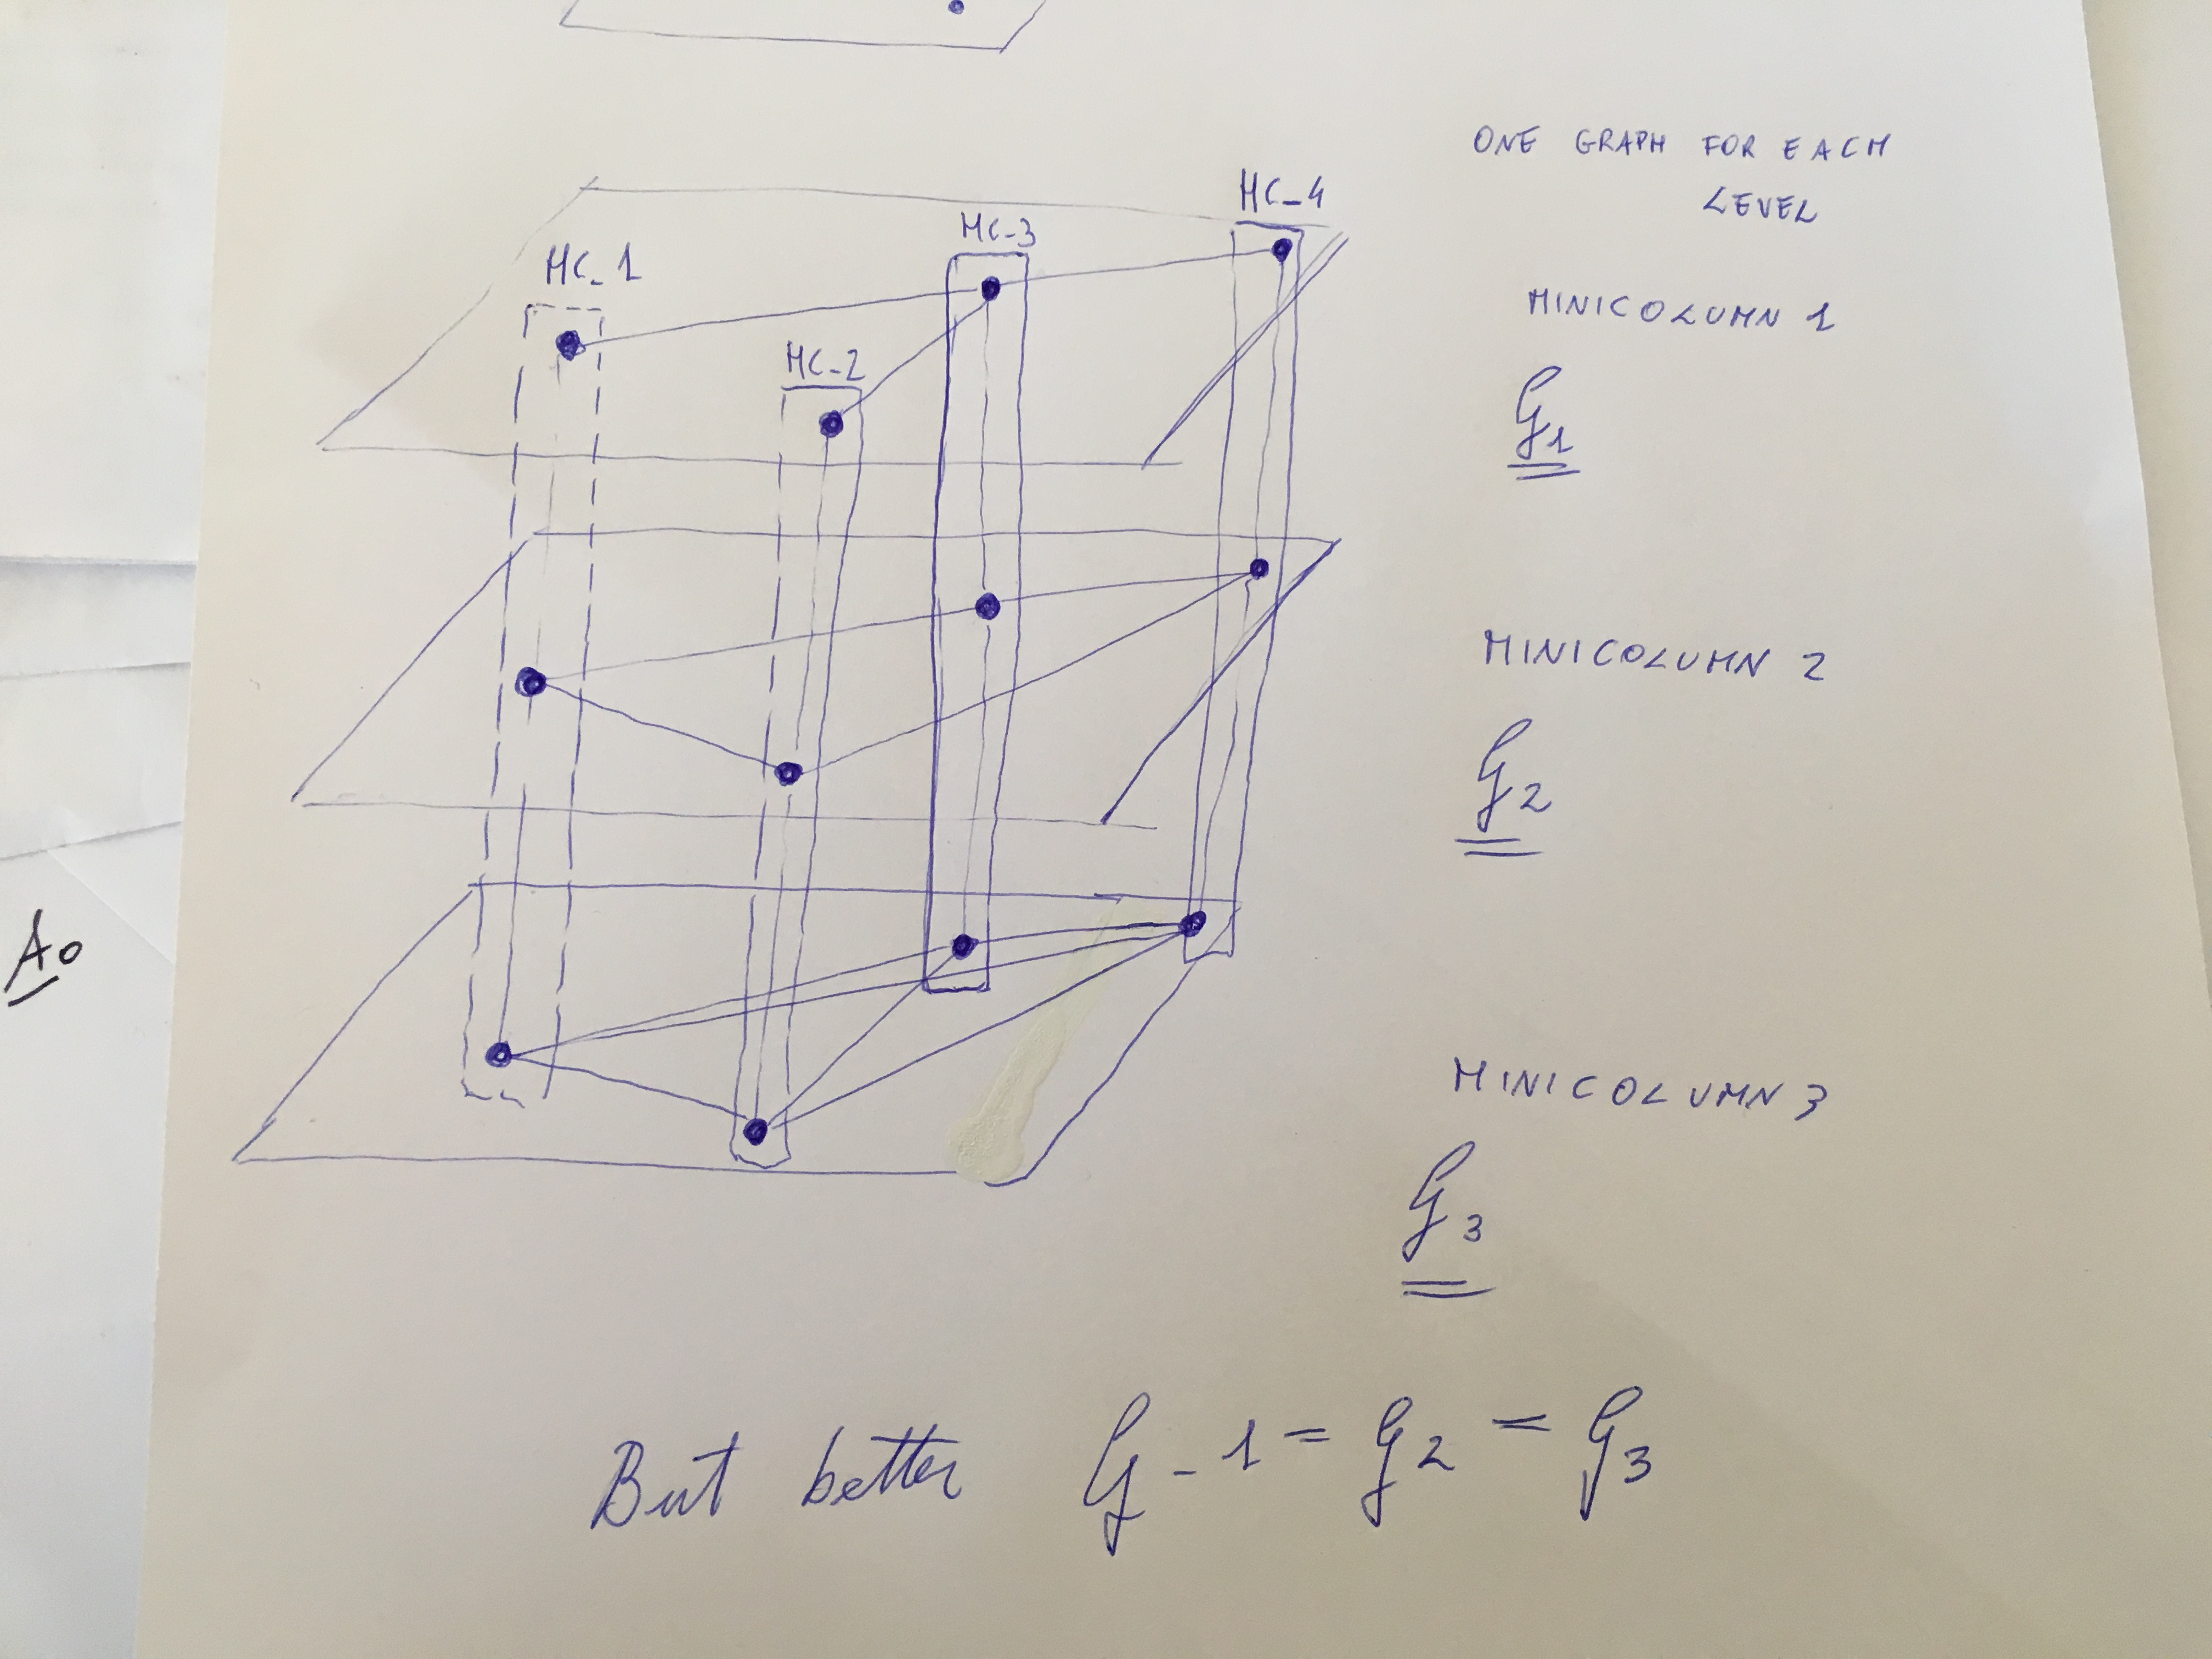
\includegraphics[width=\textwidth]{text/analysis/fig/2by2adapt/image1.jpeg}
    \caption{Simulation of system in \eqref{eq:cl_loop} with several initial conditions. $\alpha=1.5$}
    \label{fig:network_levels}
\end{figure}
